\documentclass[12pt, a4paper]{article}
\usepackage[reals]{layout} %provide \layout macro to show current page layout

\usepackage{cite}

\usepackage{listings}
\lstset{ 
  language=C++,
  morekeywords={Float_t, Int_t, Double_t, Bool_t},
  frame=tbrl,
  frameround=tttt,
  showspaces=false,
  showtabs=false,
  basicstyle=\footnotesize,
% backgroundcolor=\color{Gray},
% fillcolor=\color{Gray},
  extendedchars=true
}            
\lstloadlanguages{sh,bash,csh,[GNU]C++,[gnu]make,SQL}

\usepackage{graphicx}
\usepackage{subfigure}
\usepackage{wrapfig}

\usepackage{amsmath}            % more evironment
\usepackage{amssymb}            % more symbol

\usepackage{ifpdf}
\ifpdf
\usepackage{epstopdf} % must be put after graphicx
\usepackage[usenames,dvipsnames]{color}
\usepackage[pdftex,bookmarks=true]{hyperref}
\hypersetup{
  pdfauthor = {Jing Liu},
  pdftitle = {memo for scanning of SII},
  pdfkeywords = {pulse shape simulation},
}
\pdfadjustspacing=1 %force pdfLaTeX to use the same spacing as LaTeX
\else
\usepackage[usenames,dvips]{color}
\usepackage[ps2pdf]{hyperref}
\fi

\setlength{\oddsidemargin}{0.8cm}
\setlength{\evensidemargin}{0cm}
\setlength{\textwidth}{15cm}
\setlength{\textheight}{21cm}
\setlength{\hoffset}{0cm}
\setlength{\voffset}{0cm}

% Alter some LaTeX defaults for better treatment of floats: See p.105 % of "TeX Unbound" for suggested values. See pp. 199-200 of Lamport's % "LaTeX" book for details.

% General parameters, for ALL pages:
\renewcommand{\topfraction}{0.9} % max fraction of floats at top
\renewcommand{\bottomfraction}{0.9} % max fraction of floats at bottom

% Parameters for TEXT pages (not float pages):
\setcounter{topnumber}{2}
\setcounter{bottomnumber}{2}
\setcounter{totalnumber}{4} % 2 may work better
\renewcommand{\textfraction}{0.1} % allow minimal text w. figs

% Parameters for FLOAT pages (not text pages):
\renewcommand{\floatpagefraction}{0.7}	% require fuller float pages
% N.B.: floatpagefraction MUST be less than topfraction !!

% remember to use [htp] or [htpb] for placement
%\pagestyle{headings}

%% The lineno packages adds line numbers. Start line numbering with
%% \begin{linenumbers}, end it with \end{linenumbers}. Or switch it on
%% for the whole article with \linenumbers.
\usepackage{lineno}

%%% Local Variables: 
%%% mode: latex
%%% TeX-master: "memo"
%%% End: 


\title{Surface scanning of Siegfried II in Gerdalinchen II}

\author{Jing Liu}

\date{\today{}}

\begin{document}
\maketitle{}
\tableofcontents

\section{Size of the beam spot}
\label{s:col}
The penetrating depth of 121~keV photons in tungsten is simulated
using MaGe:
\begin{lstlisting}
  $ MaGe ~/work/gerdalinchenII/scan/collimator/r2mm/W.mac
\end{lstlisting}
The 121~keV photons are emitted isotropically outward from the center
of a tungsten sphere. The geometry is defined in file
\lstinline!Wsphere.gdml! The radius of the hits ``hitR'' weighted by
their energy ``hitE'' are plotted in Fig.~\ref{f:w121}. Most of the
121~keV photons are stopped within 1~mm. The tungsten collimator used
in the scan can collimate the 121~keV photons almost perfectly. The
size of the beam spot on the surface of Siegfried~II can be calculated
geometrically. 

\begin{figure}[fptb]
  \centering
  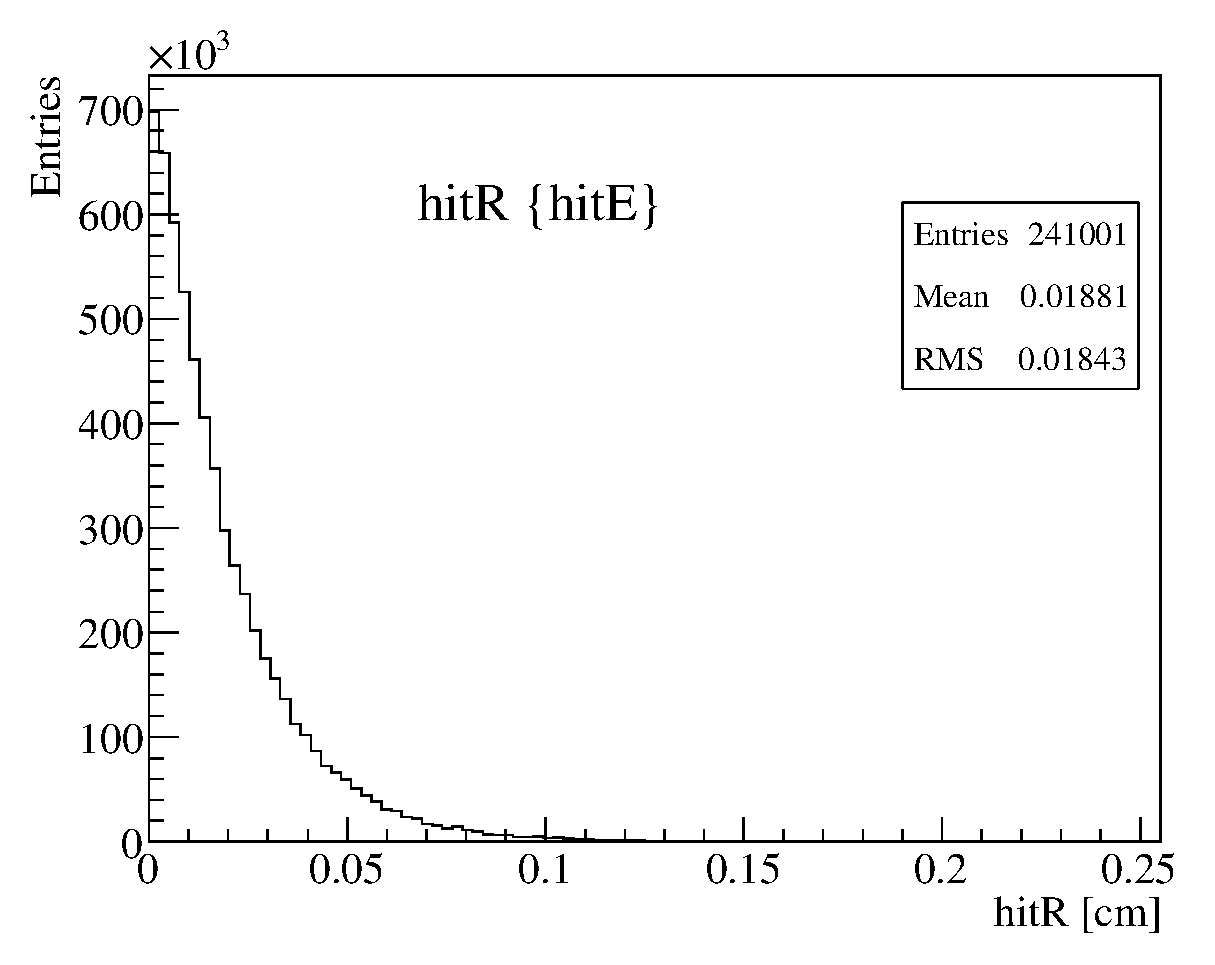
\includegraphics[width=0.5\textwidth]{w121keV}
  \caption{Penetrating depth of 121~keV photons in tungsten.}
  \label{f:w121}
\end{figure}

Figure~\ref{f:setup} showns the experimental setup. The diameter of
the beam spot $r$ on the surface of the detector can be calculated as:
\begin{equation}
  \label{e:size}
  r = (28+10.5)/28 \times 2 = 2.75 \text{ mm}.
\end{equation}

\begin{figure}[fptb]
  \centering
  \includegraphics[width=0.8\textwidth]{../../hole/occupancy/memo/segID}
  \caption{Experimental setup.}
  \label{f:setup}
\end{figure}

\end{document}

%%% Local Variables:
%%% mode: latex
%%% TeX-master: t
%%% End: 
